\documentclass[11pt,a4paper]{extarticle}
\usepackage{geometry}
 \geometry{
 a4paper,
 total={160mm,237mm},
 left=25mm,
 top=25mm,
 }
\usepackage[utf8x]{inputenc}
\usepackage[english]{babel}
\usepackage{bbm}
\usepackage[usenames]{color}
\usepackage{hyperref}
\usepackage{colortbl}
\usepackage{amsmath}
\usepackage{amssymb}
\usepackage[pdftex]{graphicx}
\usepackage{amsthm}
\usepackage{caption}
\usepackage[ruled,vlined]{algorithm2e}
\usepackage{authblk}
\usepackage{float}
\usepackage{caption}

\title{Course project \\
"Risk analysis and high-dimensional integrals"}
\author{ Nikita Puchkin, Igor Silin,Alexander Podkopaev }

\begin{document}

\maketitle

\section{Team members}

\begin{itemize}

\item Igor Silin (leader)

Igor implemented a solver for numerical solution of Black-Scholes partial differential equation.
The code can be found in 'bs\_solver.py'.
He described a background, formulated a problem and described, how to reduce it to reaction-diffusion equation as well.

\item Nikita Puchkin

Nikita implemented a solver for numerical solution of reaction-diffusion equation.
The code can be found in 'pde\_solver.py'.
He prepared description of method and algorithm in this report as well. 

\item Aleksandr Podkopaev

Alexandr found different options and tested solver for Black-Scholes partial differential equation.
He also visualized results.
The code can be found in 'visualization.py'.
He prepared a section with data and results in this report as well.

\end{itemize}

\section{Background}

Many stock prices can modelled using Brownian motion, i.e. the next state depends on the previous state plus some random event. Important statistical options (for example, option calls) can be then estimated as expectations of random process. Option is a contract which gives the owner of the option the right, but not the obligation, to buy or sell an underlying asset at a specified price on a specified date, depending on the form of the option. Two types of options are considered: call options that give the holder the right to buy an asset at a specified price on a specified date and put options that give the holder the right to sell an asset at a specified price on a specified date. The straightforward way for estimation of options is to do Monte-Carlo simulation, but it can not give high accuracy. Another way is to write down the expectation as a path integral and then approximate it by a multi-dimensional integral. More detailed description of the problem which is solved is given in the next section.

\section{Problem formulation}

Denote by $s$ the stock price and by $c(s,t)$ general option value. Then consider Black-Scholes pricing model. It is known that in that case $c$ must satisfy the following partial differential equation:

\begin{equation}
	\begin{aligned}
		&\frac{\partial c(s,t)}{\partial t} + rs \frac{\partial c(s,t)}{\partial s} + \frac12 \gamma^2 s^2 \frac{\partial^2 c(s,t)}{\partial s^2} = rc(s,t),
		\;\;\;s \in \mathbbm{R}_{+},\;\; t \in [0;\;T^{\prime}],\\
		&c(s,T^{\prime}) = g(s), \;\;\; s \in \mathbbm{R}_{+},\\
		&c(0,t) = 0, \;\;\; t \in [0;\;T^{\prime}].
	\end{aligned}
\end{equation}
Here  $r$ is the risk-free interest rate and $\gamma$ is the volatility of the stock.
This is called Black-Scholes partial differential equation. Different terminal conditions $g(s)$ corresponds to different types of derivatives (e.g. European call option). We are interested in methods of solving given PDE for different terminal conditions which are described in the next section.

\section{Data}

We've chosen several types of options when setting terminal conditions allows to solve Black-Scholes PDE analytically. Let us consider these cases.

\subsection{European call option}

The corresponding terminal function is:

\begin{equation}
    \begin{aligned}
    g(s)=\max\{s-E, 0\}
    \end{aligned}
    \end{equation}

For introducing the analytical solution, we firstly denote:

\begin{equation}
    \begin{aligned}
    d_{+}^{T^\prime}(t)=\frac{\log(\frac{s}{E})+(r+\frac{\gamma^2}{2})(T^\prime-t)}{\gamma\sqrt{T^\prime-t}}
    \end{aligned}
    \end{equation}

\begin{equation}
    \begin{aligned}
    d_{-}^{T^\prime}(t)=\frac{\log(\frac{s}{E})+(r-\frac{\gamma^2}{2})(T^\prime-t)}{\gamma\sqrt{T^\prime-t}}
    \end{aligned}
    \end{equation}

\begin{equation}
    \begin{aligned}
    \Phi(x)=\frac{1}{\sqrt{2\pi}}\int_{-\infty}^xe^{-\frac{y^2}{2}}dy
    \end{aligned}
    \end{equation}

Then the analytical solution for the case of european call is:

\begin{equation}
    \begin{aligned}
    c(s,t) = s\Phi(d_{+}^{T^\prime})-Ee^{-r(T^\prime-t)}\Phi(d_{-}^{T^\prime})
    \end{aligned}
    \end{equation}

\subsection{European put option}

The corresponding terminal function is:

\begin{equation}
    \begin{aligned}
    g(s)=\max\{E-s, 0\}
    \end{aligned}
    \end{equation}

Then the analytical solution for the case of european put option is:

\begin{equation}
    \begin{aligned}
    c(s,t) = Ee^{-r(T^\prime-t)}\Phi(-d_{-}^{T^\prime})-s\Phi(-d_{+}^{T^\prime})
    \end{aligned}
    \end{equation}

\subsection{Cash-or-nothing call option}

The corresponding terminal function is:

\begin{equation}
    \begin{aligned}
    g(s)=\begin{cases}B,&s\geq E \\ 0,&\text{otherwise}\end{cases}
    \end{aligned}
    \end{equation}

Then the analytical solution for the case of cash-or-nothing call option is:

\begin{equation}
    \begin{aligned}
    c(s,t) = Be^{-r(T^\prime-t)}\Phi(d_{-}^{T^\prime})
    \end{aligned}
    \end{equation}

\subsection{Cash-or-nothing put option}

The corresponding terminal function is:

\begin{equation}
    \begin{aligned}
    g(s)=\begin{cases}0,&s\geq E \\ B,&\text{otherwise}\end{cases}
    \end{aligned}
    \end{equation}

Then the analytical solution for the case of case of cash-or-nothing put option is:

\begin{equation}
    \begin{aligned}
    c(s,t) = Be^{-r(T^\prime-t)}\Phi(-d_{-}^{T^\prime})
    \end{aligned}
    \end{equation}

\subsection{Asset-or-nothing call option}

The corresponding terminal function is:

\begin{equation}
    \begin{aligned}
    g(s)=\begin{cases}s,&s\geq E \\ 0,&\text{otherwise}\end{cases}
    \end{aligned}
    \end{equation}

Then the analytical solution for the case of asset-or-nothing call option is:

\begin{equation}
    \begin{aligned}
    c(s,t) = s\Phi(d_{+}^{T^\prime})
    \end{aligned}
    \end{equation}

\subsection{Asset-or-nothing put option}

The corresponding terminal function is:

\begin{equation}
    \begin{aligned}
    g(s)=\begin{cases}0,&s\geq E \\ s,&\text{otherwise}\end{cases}
    \end{aligned}
    \end{equation}

Then the analytical solution for the case of case of asset-or-nothing put option is:

\begin{equation}
    \begin{aligned}
    c(s,t) =s\Phi(-d_{+}^{T^\prime})
    \end{aligned}
    \end{equation}

\section{Related work}

We implement the method based on one described in \cite{oseledets}.

\section{Scope}

The solution is based on two important steps: firstly, we reduce the initial problem to one described in related paper, secondly, we implement the method proposed in that paper to get numerical solution.

\subsection{Reduction to one-dimensional reaction-diffusion equation}

Consider variable substitution of the following type: $x=\ln s$ and $w(x,t) = c(s, t)$. Then after sequence of elementary transformations one obtains:
\begin{equation}
	\begin{aligned}
		&\frac{\partial w(x,t)}{\partial t} + \left(r-\frac{\gamma^2}{2}\right) \frac{\partial w(x,t)}{\partial x} +
		\frac12 \gamma^2 \frac{\partial^2 w(x,t)}{\partial x^2} = rw(x,t),
		\;\;\;x \in \mathbbm{R},\;\; t \in [0;\;T^{\prime}],\\
		&w(x,T^{\prime}) = g(e^x), \;\;\; x \in \mathbbm{R},\\
		&w(-\infty,t) = 0, \;\;\; t \in [0;\;T^{\prime}].
	\end{aligned}
\end{equation}
To get rid of the drift term $\left(r-\frac{\gamma^2}{2}\right) \frac{\partial w(x,t)}{\partial x}$ we introduce
\begin{equation}
	\begin{aligned}
		v(x,t) = e^{\frac{1}{\gamma^2} (r-\frac{\gamma^2}{2})x} w(x,t),
	\end{aligned}
\end{equation}
and obtain
\begin{equation}
	\begin{aligned}
		&\frac{\partial v(x,t)}{\partial t} + \frac12 \gamma^2 \frac{\partial^2 v(x,t)}{\partial x^2} =
		\left( r +  \frac{1}{2\gamma^2} \left( r-\frac{\gamma^2}{2}\right)^2 \right) v(x,t),
	 	\;\;\;x \in \mathbbm{R},\;\; t \in [0;\;T^{\prime}],\\
		&v(x,T^{\prime}) = e^{\frac{1}{\gamma^2} (r-\frac{\gamma^2}{2})x} g(e^x), \;\;\; x \in \mathbbm{R},\\
		&v(-\infty,t) = 0, \;\;\; t \in [0;\;T^{\prime}].
	\end{aligned}
\end{equation}
Introducing
$\sigma = \frac12 \gamma^2$, $V(x,t) = V = r +  \frac{1}{2\gamma^2} \left( r-\frac{\gamma^2}{2}\right)^2$ and
$f(x) = e^{\frac{1}{\gamma^2} (r-\frac{\gamma^2}{2})x} g(e^x)$  we have
\begin{equation}
	\begin{aligned}
		&-\frac{\partial v(x,t)}{\partial t} = \sigma \frac{\partial^2 v(x,t)}{\partial x^2} - V(x,t) v(x,t),
		\;\;\;x \in \mathbbm{R},\;\; t \in [0;\;T^{\prime}],\\
		&v(x,T^{\prime}) = f(x), \;\;\; x \in \mathbbm{R},\\
		&v(-\infty,t) = 0, \;\;\; t \in [0;\;T^{\prime}].
	\end{aligned}
\end{equation}


Finally, we set $u(x,t) = v(x, T^{\prime}-t)$ and obtain
\begin{equation}
	\begin{aligned}
		&\frac{\partial u(x,t)}{\partial t} = \sigma \frac{\partial^2 u(x,t)}{\partial x^2} - V(x,t) u(x,t),
		\;\;\;x \in \mathbbm{R},\;\; t \in [0;\;T^{\prime}],\\
		&v(x,0) = f(x), \;\;\; x \in \mathbbm{R},\\
		&v(-\infty,t) = 0, \;\;\; t \in [0;\;T^{\prime}].
	\end{aligned}
\end{equation}
The condition $v(-\infty,t) = 0$ will be satisfied automatically, so our partial differential equation is
\begin{equation}
	\begin{aligned}
		&\frac{\partial u(x,t)}{\partial t} = \sigma \frac{\partial^2 u(x,t)}{\partial x^2} - V(x,t) u(x,t),
		\;\;\;x \in \mathbbm{R},\;\; t \in [0;\;T^{\prime}],\\
		&u(x,0) = f(x), \;\;\; x \in \mathbbm{R}.
	\label{OseledetsForm}
	\end{aligned}
\end{equation}
This form is exactly one that is considered in Oseledets's paper.

So, when we have $g(s)$, $\gamma$, $r$, $T^{\prime}$ from our financial model, we just set
\begin{equation}
	\begin{aligned}
		f(x) = e^{\frac{1}{\gamma^2} (r-\frac{\gamma^2}{2})x} g(e^x), \;\; \sigma = \frac12 \gamma^2, \;\;\; V(x,t) = V = r +  \frac{1}{2\gamma^2} \left( r-\frac{\gamma^2}{2}\right)^2,
	\end{aligned}
\end{equation}
solve (\ref{OseledetsForm}) with this parameters, and reconstruct the desired function $c(s,t)$ as
\begin{equation}
	\begin{aligned}
		c(s,t) = w(e^x, t) = e^{-\frac{1}{\gamma^2} (r-\frac{\gamma^2}{2})\ln s} v(\ln s, t) = e^{-\frac{1}{\gamma^2} (r-\frac{\gamma^2}{2})\ln s} u(\ln s, T^{\prime} - t).
	\end{aligned}
\end{equation}

\subsection{Description of algorithm and PDE solver}

We implement a solver for numerical solution of PDE

\begin{equation}
     \begin{aligned}
     \nonumber
        %\left\{
        & \frac\partial{\partial t} u(x, t) = \sigma \frac{\partial^2}{\partial x^2} u(x, t) - V(x, t) u(x, t), \quad t\in [0, T], \, x\in \mathbb R \\
        & u(x, 0) = f(x)
        %\right.
     \end{aligned}
\end{equation}

In this section we use the same idea as described in \cite{oseledets}.
The exact solution is given by the Feynman-Kac formula

\begin{equation}
    \begin{aligned}
    \nonumber
        u(x, T) = \int\limits_{C\{x, 0; T\}} f(\xi(T)) \exp\left\{ -\int\limits_0^T V(\xi(\tau), T-\tau) d\tau \right\} \mathcal D_\xi,
    \end{aligned}
\end{equation}
where the integration is done over the set $C\{x, 0; T\}$ of all continuous paths $\xi(T) : [0, T] \rightarrow \mathbb R$ from the Banach space $\Xi([0, T], \mathbb R)$ starting at $\xi(0) = x$ and stopping at arbitrary endpoints at time $T$.
$\mathcal D_\xi$ is the Wiener measure and $\xi(t)$ is the Wiener process.

For numerical computation one can break the time range $[0, T]$ into $n$ intervals by points
\begin{equation}
    \begin{aligned}
    \nonumber
        \tau_k = k \delta t, \qquad 0 \leq k < n, \qquad n: \, \tau_n = T
    \end{aligned}
\end{equation}
The average path of a Brownian particle $\xi(\tau_k)$ after $k$ steps is defined as
\begin{equation}
    \begin{aligned}
    \nonumber
        \xi^{(k)} = \xi(\tau_k) = x + \xi_1 + \dots + \xi_k,
    \end{aligned}
\end{equation}
where every random step $\xi_i$, $1 \leq i \leq k$, is independently taken from a normal distribution $\mathcal N(0, 2\sigma\delta t)$.
By definition $\xi^{(0)} = x$.

On the introduced uniform grid one approximates
\begin{equation}
    \begin{aligned}
    \nonumber
        \Lambda(T) = \int\limits_0^T V(\xi(\tau), T - \tau) d\tau \simeq \sum\limits_{i=0}^n w_i V_i^{(n)} \delta t, \qquad V_i^{(n)} \equiv V(\xi(\tau_i), \tau_{n-i}),
    \end{aligned}
\end{equation}
where the set of weights $\{w_i\}_{i=0}^n$ is taken according to trapezoid rule or Simpson rule.
Then
\begin{equation}
    \begin{aligned}
    \nonumber
    \exp\{-\Lambda(T)\} \simeq \prod\limits_{i=0}^n \exp\{-w_i V_i^(n) \delta t
    \end{aligned}
\end{equation}
The Wiener measure transforms to $n$\/-dimensional measure
\begin{equation}
    \begin{aligned}
    \nonumber
    \mathcal D_\xi^{(n)} = \left( \frac\lambda\pi \right)^{\frac n2} \prod\limits_{k=1}^n \exp\{-\lambda \xi_k^2\} d\xi_k, \qquad \lambda = \frac1{4\sigma \delta t},
    \end{aligned}
\end{equation}
and a numerical approximation of the exact solution can be written in the form
\begin{equation}
    \begin{aligned}
    \nonumber
    u^{(n)}(x, T) = \int\limits_{-\infty}^\infty \mathcal D_{xi} f(\xi^{(n)}) \prod\limits_{i=0}^n e^{-w_i v_i^{(n)}\delta t}
    \end{aligned}
\end{equation}

The multidimensional integral can be represented in terms of $n$ one-dimensional convolutions.
Define
\begin{equation}
    \begin{aligned}
    \nonumber
    F_k^{(n)}(x) = \sqrt{\frac\lambda\pi} \int\limits_{-\infty}^{\infty} \Phi_{k+1}^{(n)}(x+\xi) e^{-\lambda \xi^2} d\xi, \qquad x\in \mathbb R, \quad k = n, n-1, \dots, 1,
    \end{aligned}
\end{equation}
where
\begin{equation}
    \begin{aligned}
    \nonumber
    \Phi_{k+1}^{(n)}(x) = F^{(n)}_{k+1}(x)\exp\{-w_k V(x, \tau_{n-k}) \delta t,
    \end{aligned}
\end{equation}
and
\begin{equation}
    \begin{aligned}
    \nonumber
    F^{(n)}(x)_{n+1} = f(x)
    \end{aligned}
\end{equation}
Then the numerical solution is given by formula
\begin{equation}
    \begin{aligned}
    \nonumber
    u^{(n)}(x, T) = F_1^{(n)}(x) e^{-w_0 V(x, T) \delta t}
    \end{aligned}
\end{equation}

Since $F_k^{(n)}(x)$ is represented as integral over all real values, it is replaced by an integral over a segment
\begin{equation}
    \begin{aligned}
    \nonumber
    F_k^{(n)}(x) \simeq \tilde F_k^{(n)}(x) = \sqrt{\frac\lambda\pi} \int\limits_{-a_x}^{a_x - h_x} \Phi_{k+1}^{(n)}(x + \xi) e^{-\lambda \xi^2} d\xi
    \end{aligned}
\end{equation}

The function $F_k^{(n)}(x)$ is computed on the uniform mesh
\begin{equation}
    \begin{aligned}
    \nonumber
    x_i^{(k)} = -ka_x + ih_x, \qquad 0 \leq i \leq kM, \qquad h_x = \frac{a_x}{N_x}, \qquad M = 2N_x
    \end{aligned}
\end{equation}
and the integration mesh is taken with the same step $h_x$
\begin{equation}
    \begin{aligned}
    \nonumber
    \xi_j = -a_x + jh_x, \qquad 0 \leq j < M
    \end{aligned}
\end{equation}

Then
\begin{equation}
    \begin{aligned}
    \nonumber
    \tilde F_k^{(n)} (x_i^{(k)}) \simeq \sum\limits_{j=0}^{M-1} \mu_j \Phi_{k+1}^{(n)}(x_{i+j}^{(k+1)} p(\lambda, \xi_j), \qquad p(\lambda, \xi) = \sqrt{\frac\lambda\pi e^{-\lambda \xi^2}} \\
    \Phi_{k+1}^{(n)}(x_i^{(k+1)} = \tilde F_{k+1}^{(n)}(x_i^{(k+1)} \exp\{ -w_k V(x_i^{(k+1)}, \tau_{n-k}) \delta t
    \end{aligned}
\end{equation}
or in the matrix form
\begin{equation}
    \begin{aligned}
    \nonumber
    \tilde F_k^{(n)} = \Phi_{k+1}^{(n)} \circ \tilde\mu, \qquad \tilde\mu_j = \mu_j p(\lambda, \xi_j) \\
    \Phi_{k+1}^{(n)} = \tilde F_{k+1}^{(n)} \exp\{ -w_k V(x^{(k+1)}, \tau_{n-k}) \delta t,
    \end{aligned}
\end{equation}
where $a\circ b$ denotes a convolution of vectors $a \in \mathbb R^m$ and $b \in \mathbb R^k$, i. e. a vector $c \in \mathbb R^{m+k-1}$, such that
\begin{equation}
    \begin{aligned}
    \nonumber
    c_i = \sum\limits_{j=0}^{k-1} a_{i+j}b_j, \quad a_i = 0,\, \forall i: (i < 0) \bigvee (i \geq m)
    \end{aligned}
\end{equation}

The algorithm for computation of $u^{(n)}(x, T)$ is following.

\begin{enumerate}
    \item Given $T$, choose a time step $\delta t$ and the number of steps $n = \frac T{\delta t}$.
    \item Create 1D array $\tau$ of size $n$, $\tau_i = i \delta t$.
    \item Create 1D array $w$ of size $(n+1)$, corresponding to the set of weights in trapezoid or Simpson rule.
    \item Choose $a_x$, size of coordinate grid $M = 2N_x$ and a coordinate step $h_x = \frac{a_x}{N_x}$.
    \item Initialize 1D array $\tilde F_{n+1}^{(n)}$ of size $(n+1)M$, where $F_{n+1}^{(n)} = f(x)$ and $x_i = -(n+1)a_x + ih_x$, $0 \leq i < (n+1)M$.
    \item For $k = n, n-1, \dots, 1$ do
        \begin{enumerate}
        \item Create 1D array $x^{(k+1)}$ of size $(k+1)M$, $x_i^{(k+1)} = -(k+1)a_x + ih_x$, $0 \leq i < (k+1)M$
        \item Create 1D array of size $(k + 1)M$ $e^{-w_k V(x^{(k)}, \tau_{n-k}) \delta t}$.
        \item Create 1D array $\Phi_{k+1}^{(n)} = F_{k+1}^{(n)} \odot e^{-w_k V(x^{(k+1)}, \tau_{n-k}) \delta t}$.
        \item Create 1D array $\mu$ of size $M+1$, corresponding to the set of weights.
        \item Create 1D array $\xi$ of size $M+1$, where $\xi_j = -a_x + jh_x$, $0 \leq j < M+1$.
        \item Create 1D array $\tilde\mu = \mu \odot p(\lambda, \xi)$.
        \item Compute convolution $\tilde F_k^{(n)} = \Phi_{k+1}^{(n)} \circ \tilde\mu$. $\tilde F_k^{(n)}$ is 1D array of size $kM$.
        \end{enumerate}
    \item Create 1D array $x^{(1)}$ of size $M$, $x_i^{(1)} = -a_x + ih_x$, $0 \leq i < M$
    \item Create 1D array of size $M$ $e^{-w_0 V(x^{(1)}, T) \delta t}$.
    \item Compute the numerical solution $u^{(n)} = F_1^{(n)} \odot e^{-w_0 V(x^{(1)}, T) \delta t}$.

\end{enumerate}

The proposed algorithm is implemented in class 'PDE\_Solver'.

\section{Evalution}

To measure the quality of the proposed method, we consider cases when Black-Scholes PDE can be solved analytically. Hence, to measure the quality of the obtained solution, we will simply compare numerical solutions given by the method and the analytical ones.

\section{Results}

For each of the cases we present 3 plots: the plot for the numerical solution, the plot for analytical solution and, finally, the plot which describes the difference between numerical and analytical solution. The red line on the plots stands for terminal condition $g(s)$ in each case.

\subsection{European call option}

\begin{minipage}{\linewidth}
      \centering
      \begin{minipage}{0.29\linewidth}
          \begin{figure}[H]
              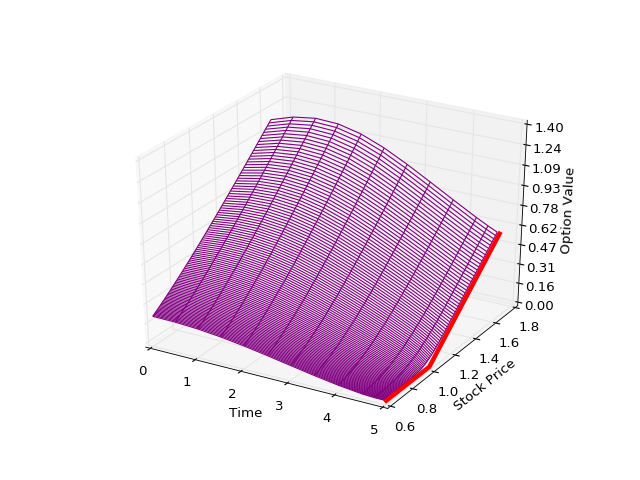
\includegraphics[width=\linewidth]{Figures/eu-call-num}
              \caption{Numerical solution}
          \end{figure}
      \end{minipage}
      \hspace{0.04\linewidth}
      \begin{minipage}{0.29\linewidth}
          \begin{figure}[H]
              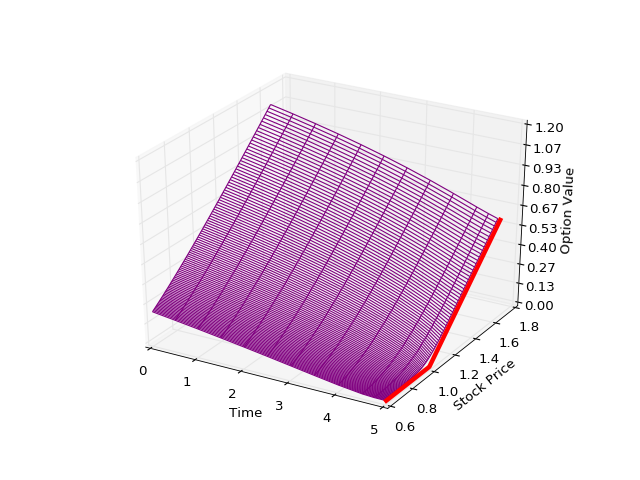
\includegraphics[width=\linewidth]{Figures/eu-call-analyt}
              \caption{Analytical solution}
          \end{figure}
      \end{minipage}
      \hspace{0.04\linewidth}
      \begin{minipage}{0.29\linewidth}
          \begin{figure}[H]
              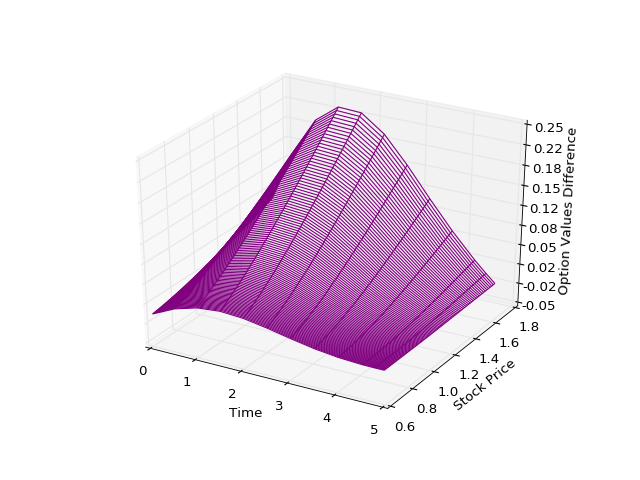
\includegraphics[width=\linewidth]{Figures/eu-call-dif}
              \caption{Difference between solutions}
          \end{figure}
      \end{minipage}
\end{minipage}

\subsection{European put option}

\begin{minipage}{\linewidth}
      \centering
      \begin{minipage}{0.29\linewidth}
          \begin{figure}[H]
              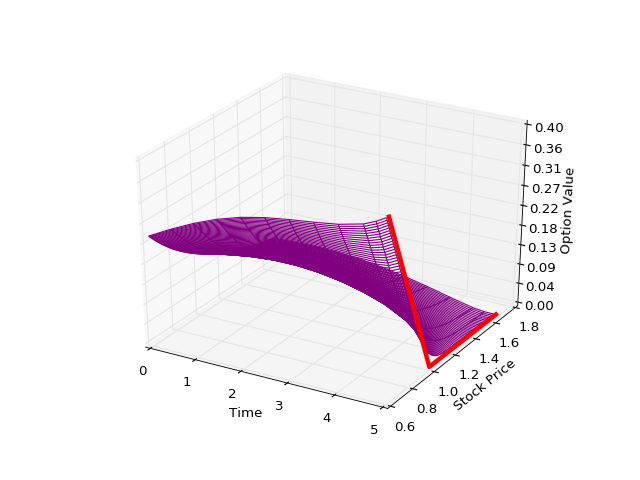
\includegraphics[width=\linewidth]{Figures/eu-put-num}
              \caption{Numerical solution}
          \end{figure}
      \end{minipage}
      \hspace{0.04\linewidth}
      \begin{minipage}{0.29\linewidth}
          \begin{figure}[H]
              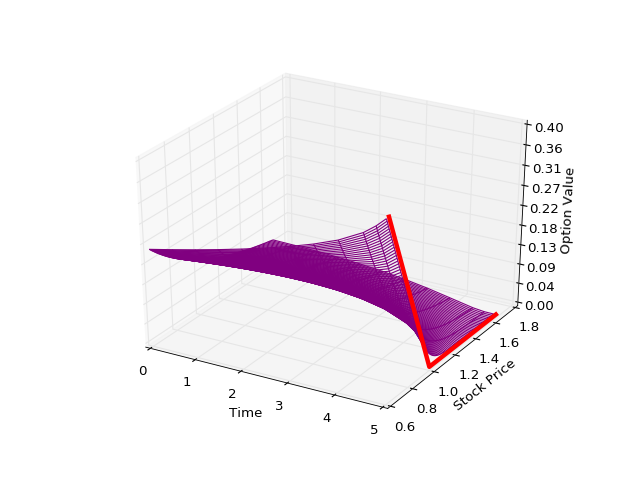
\includegraphics[width=\linewidth]{Figures/eu-put-analyt}
              \caption{Analytical solution}
          \end{figure}
      \end{minipage}
      \hspace{0.04\linewidth}
      \begin{minipage}{0.29\linewidth}
          \begin{figure}[H]
              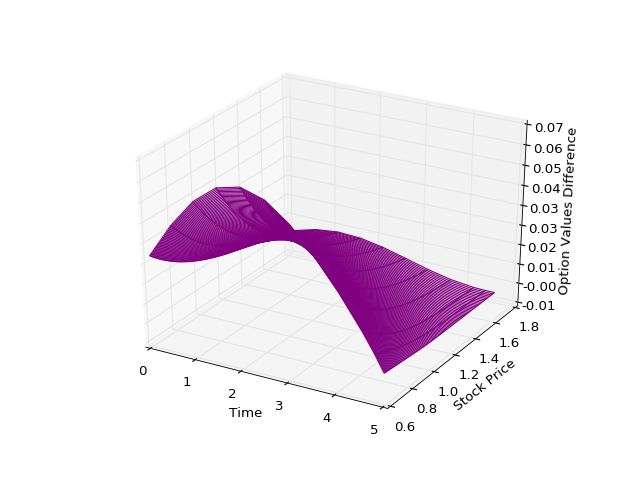
\includegraphics[width=\linewidth]{Figures/eu-put-dif}
              \caption{Difference between solutions}
          \end{figure}
      \end{minipage}
\end{minipage}

\subsection{Cash-or-nothing call option}

\begin{minipage}{\linewidth}
      \centering
      \begin{minipage}{0.29\linewidth}
          \begin{figure}[H]
              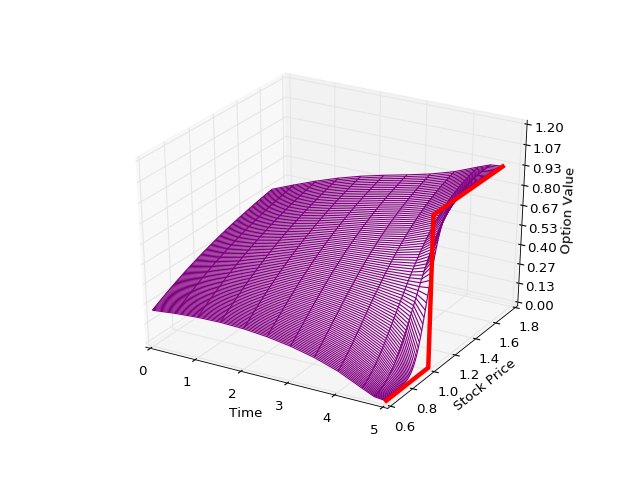
\includegraphics[width=\linewidth]{Figures/c-o-n-call-num}
              \caption{Numerical solution}
          \end{figure}
      \end{minipage}
      \hspace{0.04\linewidth}
      \begin{minipage}{0.29\linewidth}
          \begin{figure}[H]
              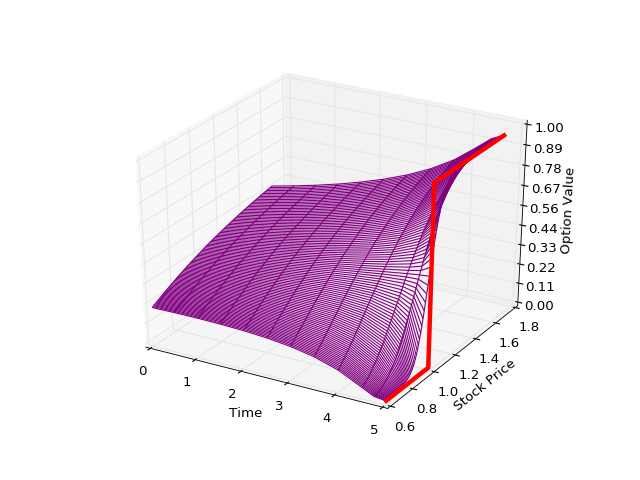
\includegraphics[width=\linewidth]{Figures/c-o-n-call-analyt}
              \caption{Analytical solution}
          \end{figure}
      \end{minipage}
      \hspace{0.04\linewidth}
      \begin{minipage}{0.29\linewidth}
          \begin{figure}[H]
              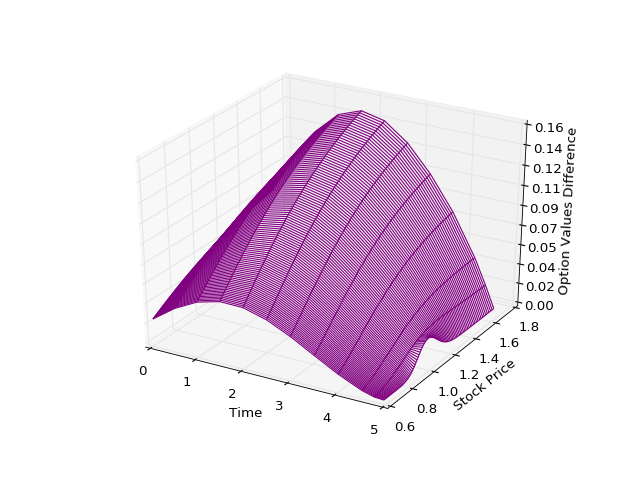
\includegraphics[width=\linewidth]{Figures/c-o-n-call-dif}
              \caption{Difference between solutions}
          \end{figure}
      \end{minipage}
\end{minipage}

\subsection{Cash-or-nothing put option}

\begin{minipage}{\linewidth}
      \centering
      \begin{minipage}{0.29\linewidth}
          \begin{figure}[H]
              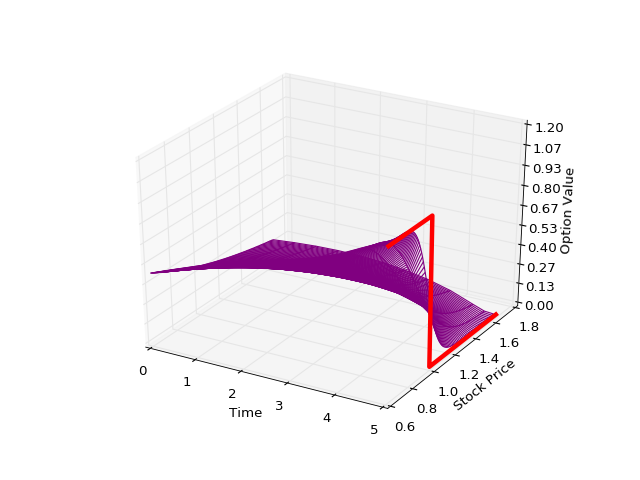
\includegraphics[width=\linewidth]{Figures/c-o-n-put-num}
              \caption{Numerical solution}
          \end{figure}
      \end{minipage}
      \hspace{0.04\linewidth}
      \begin{minipage}{0.29\linewidth}
          \begin{figure}[H]
              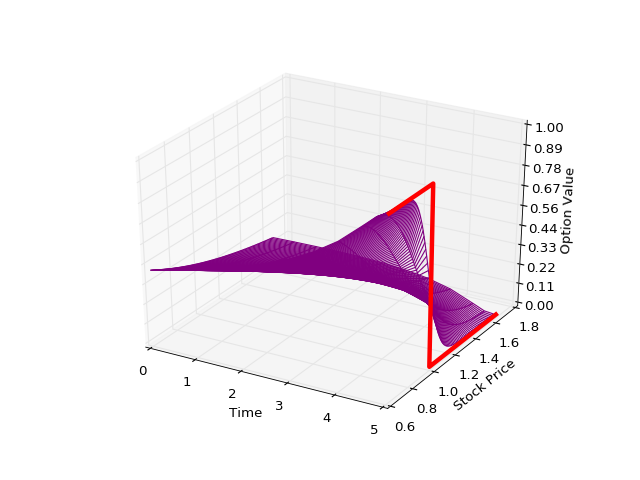
\includegraphics[width=\linewidth]{Figures/c-o-n-put-analyt}
              \caption{Analytical solution}
          \end{figure}
      \end{minipage}
      \hspace{0.04\linewidth}
      \begin{minipage}{0.29\linewidth}
          \begin{figure}[H]
              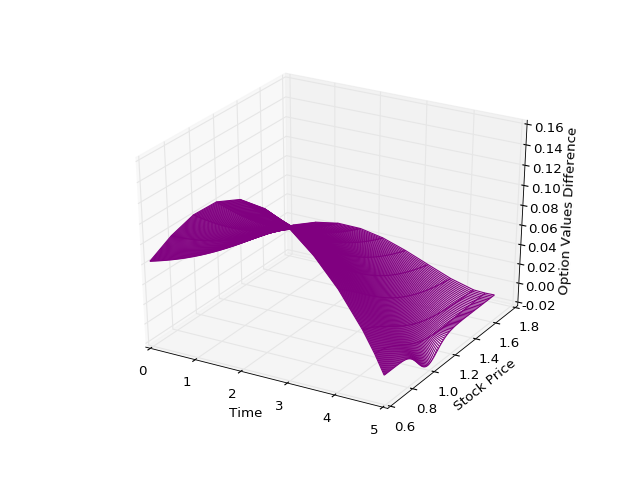
\includegraphics[width=\linewidth]{Figures/c-o-n-put-dif}
              \caption{Difference between solutions}
          \end{figure}
      \end{minipage}
\end{minipage}

\subsection{Asset-or-nothing call option}

\begin{minipage}{\linewidth}
      \centering
      \begin{minipage}{0.29\linewidth}
          \begin{figure}[H]
              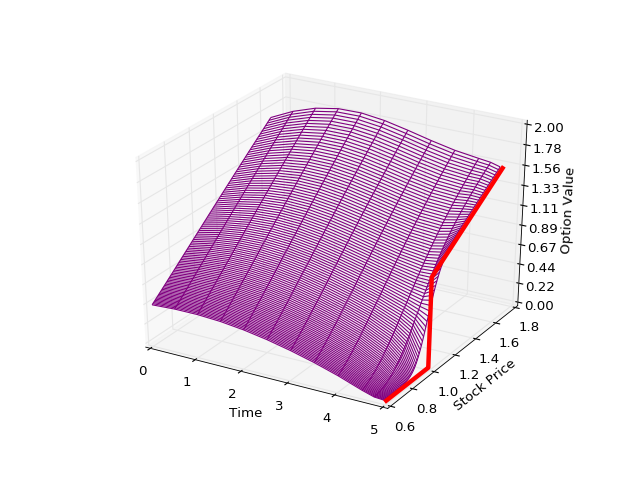
\includegraphics[width=\linewidth]{Figures/a-o-n-call-num}
              \caption{Numerical solution}
          \end{figure}
      \end{minipage}
      \hspace{0.04\linewidth}
      \begin{minipage}{0.29\linewidth}
          \begin{figure}[H]
              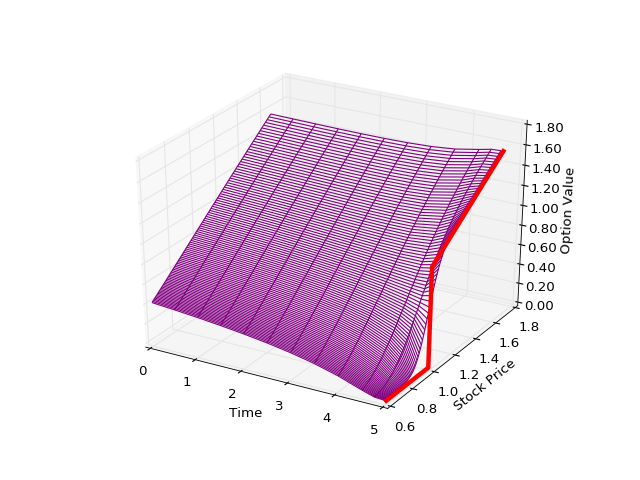
\includegraphics[width=\linewidth]{Figures/a-o-n-call-analyt}
              \caption{Analytical solution}
          \end{figure}
      \end{minipage}
      \hspace{0.04\linewidth}
      \begin{minipage}{0.29\linewidth}
          \begin{figure}[H]
              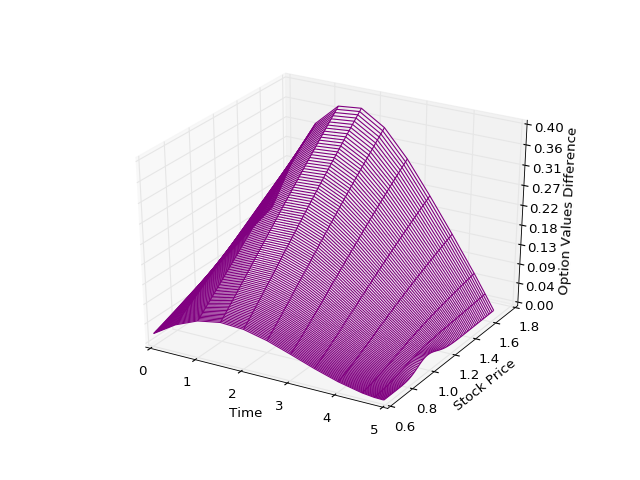
\includegraphics[width=\linewidth]{Figures/a-o-n-call-dif}
              \caption{Difference between solutions}
          \end{figure}
      \end{minipage}
\end{minipage}

\subsection{Asset-or-nothing put option}

\begin{minipage}{\linewidth}
      \centering
      \begin{minipage}{0.29\linewidth}
          \begin{figure}[H]
              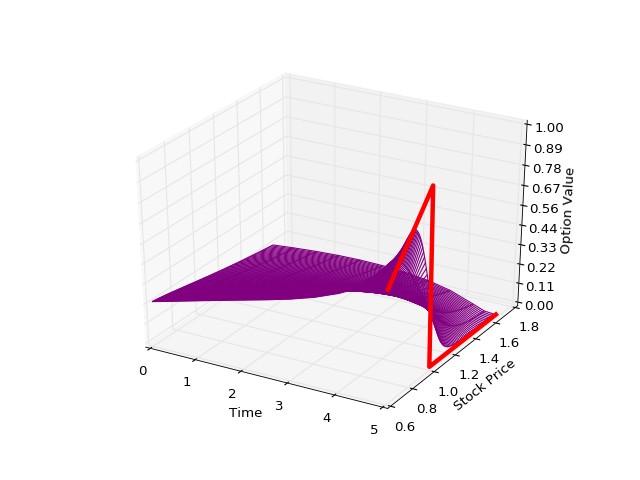
\includegraphics[width=\linewidth]{Figures/a-o-n-put-num}
              \caption{Numerical solution}
          \end{figure}
      \end{minipage}
      \hspace{0.04\linewidth}
      \begin{minipage}{0.29\linewidth}
          \begin{figure}[H]
              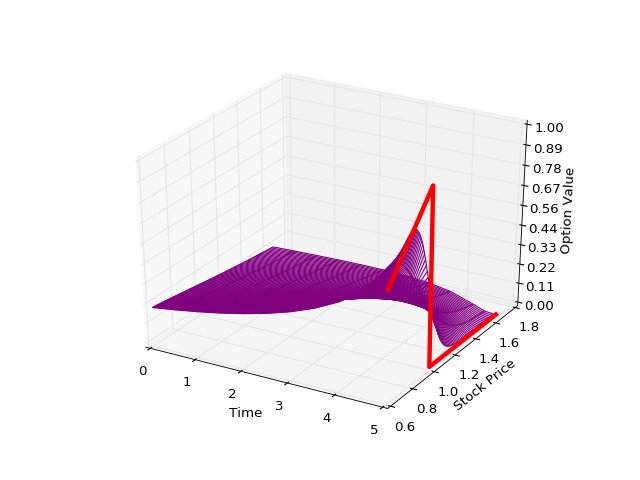
\includegraphics[width=\linewidth]{Figures/a-o-n-put-analyt}
              \caption{Analytical solution}
          \end{figure}
      \end{minipage}
      \hspace{0.04\linewidth}
      \begin{minipage}{0.29\linewidth}
          \begin{figure}[H]
              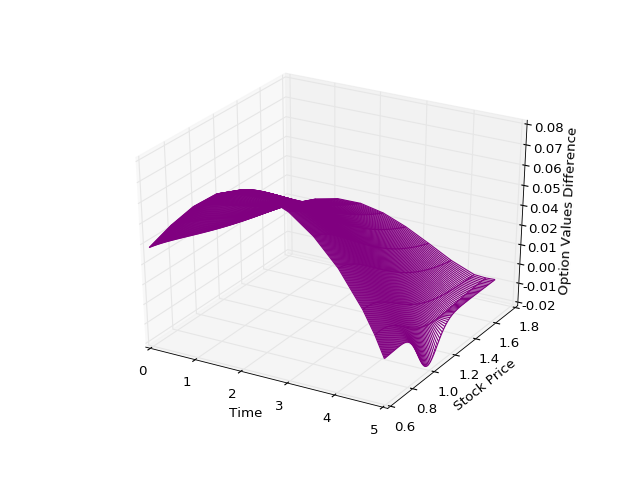
\includegraphics[width=\linewidth]{Figures/a-o-n-put-dif}
              \caption{Difference between solutions}
          \end{figure}
      \end{minipage}
\end{minipage}

\section{Conclusion}

During this work we faced the following problem: when we used substitution $s = e^x$, a function in initial conditions became to grow exponentially in $x$, while it grew linearly in $s$.
When we took a large number of time steps $n$, at the first step we had to find value of initial conditions at points with large coordinates and obtained an overflow.
Thus, we were prohibited to take large numbers of steps and, consequently, accuracy of our computations suffered.
Moreover, since $n$ was small we did not use low-rank approximation technique, because it was aimed to accelerate computations with insignificant loss of accuracy, while we were mostly interested in accurate solution.
We think, that this restriction is caused by specificity of our problem and the method proposed in \cite{oseledets} is inappropriate for this problem.
We think, it will be better to build a stable difference scheme for Black-Scholes PDE and not to make the substitution $s = e^x$.

\renewcommand{\refname}{References}
\begin{thebibliography}{9}
    \bibitem{oseledets} A low-rank approach to the computation of path integrals. M.S. Litsarev, I.V. Oseledets, 2015.
\end{thebibliography}
\end{document}
